\section{Web服务客户端管理器}
Cytoscape 2.6的一项新功能就是Web服务客户端管理器(Web Service Client Manager)。这是一个用于管理Cytoscape中各种Web服务的框架。通过Web服务客户端,用户可以方便地访问各种远程数据资源。

\subsection{什么是Web服务?}
Web服务是网络上一种标准化的,平台无关的交互机制。现在主流的生物数据库都通过Web服务API发布数据。
\begin{itemize}
\item 生物Web服务清单:http://taverna.sourceforge.net/services
\item EBI的Web服务:http://www.ebi.ac.uk/Tools/webservices/
\end{itemize}

开发人员可以编写程序访问这些服务。Cytoscape用这个框架开发了一些简单的Web服务客户端。Cytoscape支持的Web服务包括:
\begin{itemize}
\item PSICQUIC:生物相互作用数据的标准Web服务。截止2010年七月,PSICQUIC支持以下数据:
\begin{itemize}
\item  APID
\item    ChEMBL
\item    BioGrid
\item    InnateDB
\item    DIP
\item    IntAct
\item    MatrixDB
\item    MPIDB
\item    Reactome
\item    Reactome-FIs
\item    MINT
\item    iRefIndex
\item    STRING 
\end{itemize}
\item Pathway Commons:访问多种集成数据集的门户,包括Reactome, IntAct, HPRD, HumanCyc, MINT, the MSKCC Cancer Cell Map, 和NCI/Nature Pathway Interaction数据库。
\item NCBI Entrez Gene:关于基因的公共数据,包括注释、序列和相互作用。
\item Biomart:开源生物数据库引擎。可用于ID和名称的映射。
\end{itemize}

所有的这些客户端都有相应的插件,用户可以在插件管理器(Plugin Manager)中安装。

在下面几节中,我们会学习如何从外部数据库导入网络。

\section{快速入门}
首先,选择File$\rightarrow$Import$\rightarrow$Networks from web services\ldots

\centerline{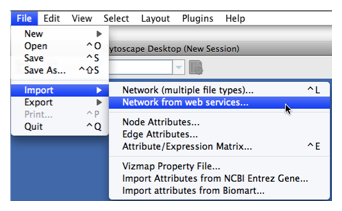
\includegraphics[width=.5\textwidth]{images/file_import.png}}

\centerline{\framebox{提示:从Web服务导入网络,见\href{http://cbio.mskcc.org/~cerami/cytoscape/CytoWebServices.mov}{动画演示}。}}

\section{例子1:从IntAct获取蛋白质相互作用网络}
\begin{itemize}
\item 选择:File$\rightarrow$Import$\rightarrow$Network from web services\ldots
\item 从下拉菜单中选择IntAct Web Service Client。
\item 输入一个或多个搜索词,例如BRCA1。
\item 点击Search按键。
\end{itemize}

\centerline{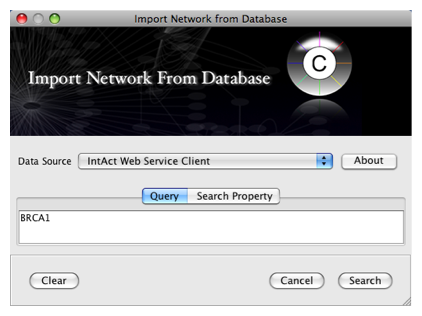
\includegraphics[width=.5\textwidth]{images/intact_import.png}}

在完成相互作用数据的下载后,BRCA1的网络就会导入Cytoscape并显示。

\centerline{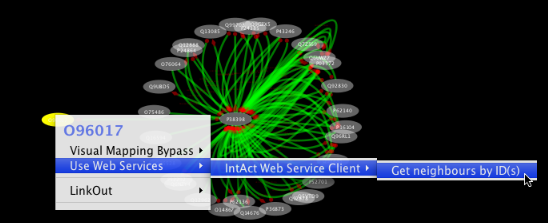
\includegraphics[width=.5\textwidth]{images/node_context2.png}}

{\bf 提示:扩展网络:}很多Cytoscape Web服务都在节点的弹出菜单中提供了一些选项。在节点上点击鼠标右键,选择``Use Web Service''。例如,在上面的截图中,我们从IntAct加载了BRCA1的网络,然后选择将节点的邻居节点添加到网络中。


\section{例子2:从NCBI Entrez Gene获取蛋白质相互作用网络}
在NCBI Entrez Gene记录中,有一段信息叫做interaction。NCBI Web服务客户端就是利用这段信息来构建网络。
\begin{itemize}
\item 选择:File$\rightarrow$Import$\rightarrow$Network from web services\ldots
\item 从下拉菜单中选择NCBI Web Service Client。
\item 输入关键字。例如,human muscular dystrophy(人类肌肉萎缩)
\item 点击Search按钮。
\end{itemize}

\centerline{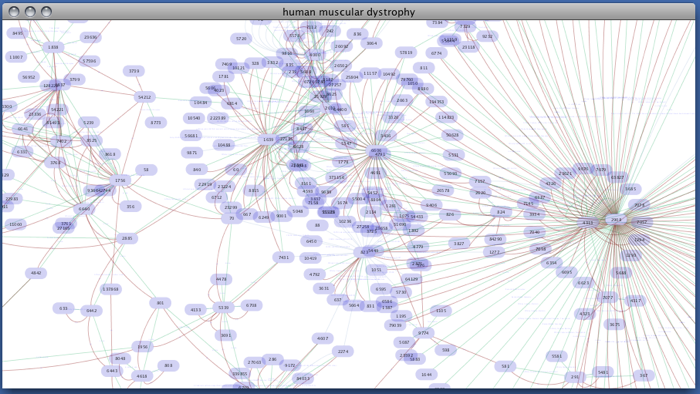
\includegraphics[width=.7\textwidth]{images/entrez_import.png}}

从Entrez Gene数据生成的网络:上图中的网络是从匹配human muscular dystrophy的interaction数据中生成的。边的颜色表示数据的来源(BIND、BioGRID或HPRD)。

{\bf 注意:}因为NCBI客户端需要从海量的数据中抽取相互作用数据,所以它需要较长的时间(30秒到5分钟,取决于机器性能和网速)来导入大量的相互作用数据。


\section{例子3:从Pathway Commons获取通路和网络}


\section{未来发展方向}

\section{从外部数据库导入属性}
\subsection{例子1:从BioMart导入ID和注释}
\subsection{例子2:从NCBI Entrez Gene数据库导入注释}

\section{在工作流中使用多个服务}
\subsection{例子:导入和注释网络}

